\documentclass[a4paper, 12pt]{article}
\usepackage[utf8]{inputenc}
\usepackage{listings}
\usepackage{graphicx}
\title{Classifying car price ranges}
\author{Sivert M. Skarning}
\date{Mai 2019}
\begin{document}
\maketitle
\clearpage

\section{Introduction}
\subsection{Problem set}
Today everything is moving online. Advertising your car by using services online is very common. So how much is your car worth? How do you categorize the price range of your car? This project focuses on how to predict the value of cars, based the car features.

The data set chosen for this project is the car evaluation data set created by Marko Bohanec. This data set contains information about 1728 cars.

\begin{itemize}
  \item buying: vhigh, high, med, low.
  \item maint: vhigh, high, med, low.
  \item doors: 2, 3, 4, 5more.
  \item persons: 2, 4, more.
  \item lug-boot: small, med, big.
  \item safety: low, med, high.
  \item Acceptability: unnac, acc, good, v-good
\end{itemize}

Based on maintenance costs, number of doors, how many persons that fits in the car, boot size, acceptability and safety rating we will try to make a model that predicts the buying price of the car. The model will use 6 predictors to classify which class the car is in. The predictors are maintenance, number of doors, number of persons that can fit in the car, luggage size, acceptability and safety.


\subsection{Data set}
\paragraph{Usage}
The car evaluation has been referenced in many scientific papers. Amongst the most noteworthy are:
\begin{itemize}
\item MML Inference of Decision Graphs with Multi-way Joins and Dynamic Attributes \cite{mml-interference}
\item Stopping Criterion for Boosting-Based Data Reduction Techniques: from Binary to Multi class Problem \cite{boosting}
\item Impact of learning set quality and size on decision tree performance \cite{learning-set}
\end{itemize}

The data set was used as an example for displaying multi attribute decision-making \cite{dataset-usage}.

\paragraph{Generation}
According to Bohanec the Car evaluation data set was created from a hierarchical decision model. This model was created for the demonstration of a decision making software called DEX \cite{dataset}.

\section{Data Pre-processing}
\subsection{Feature Extraction}
Data reduction is about removing predictors to get a smaller and simpler data-set to work with. I decided to use PCA for feature exctraction in order to simplify my data set and still capture much of the variance in the data-set. The way PCA works is that it finds predictors that are highly correlated and tries to create linear combinations of them. These linear combinations capture all of the needed information.

  \begin{figure}[h]
    \centering 
    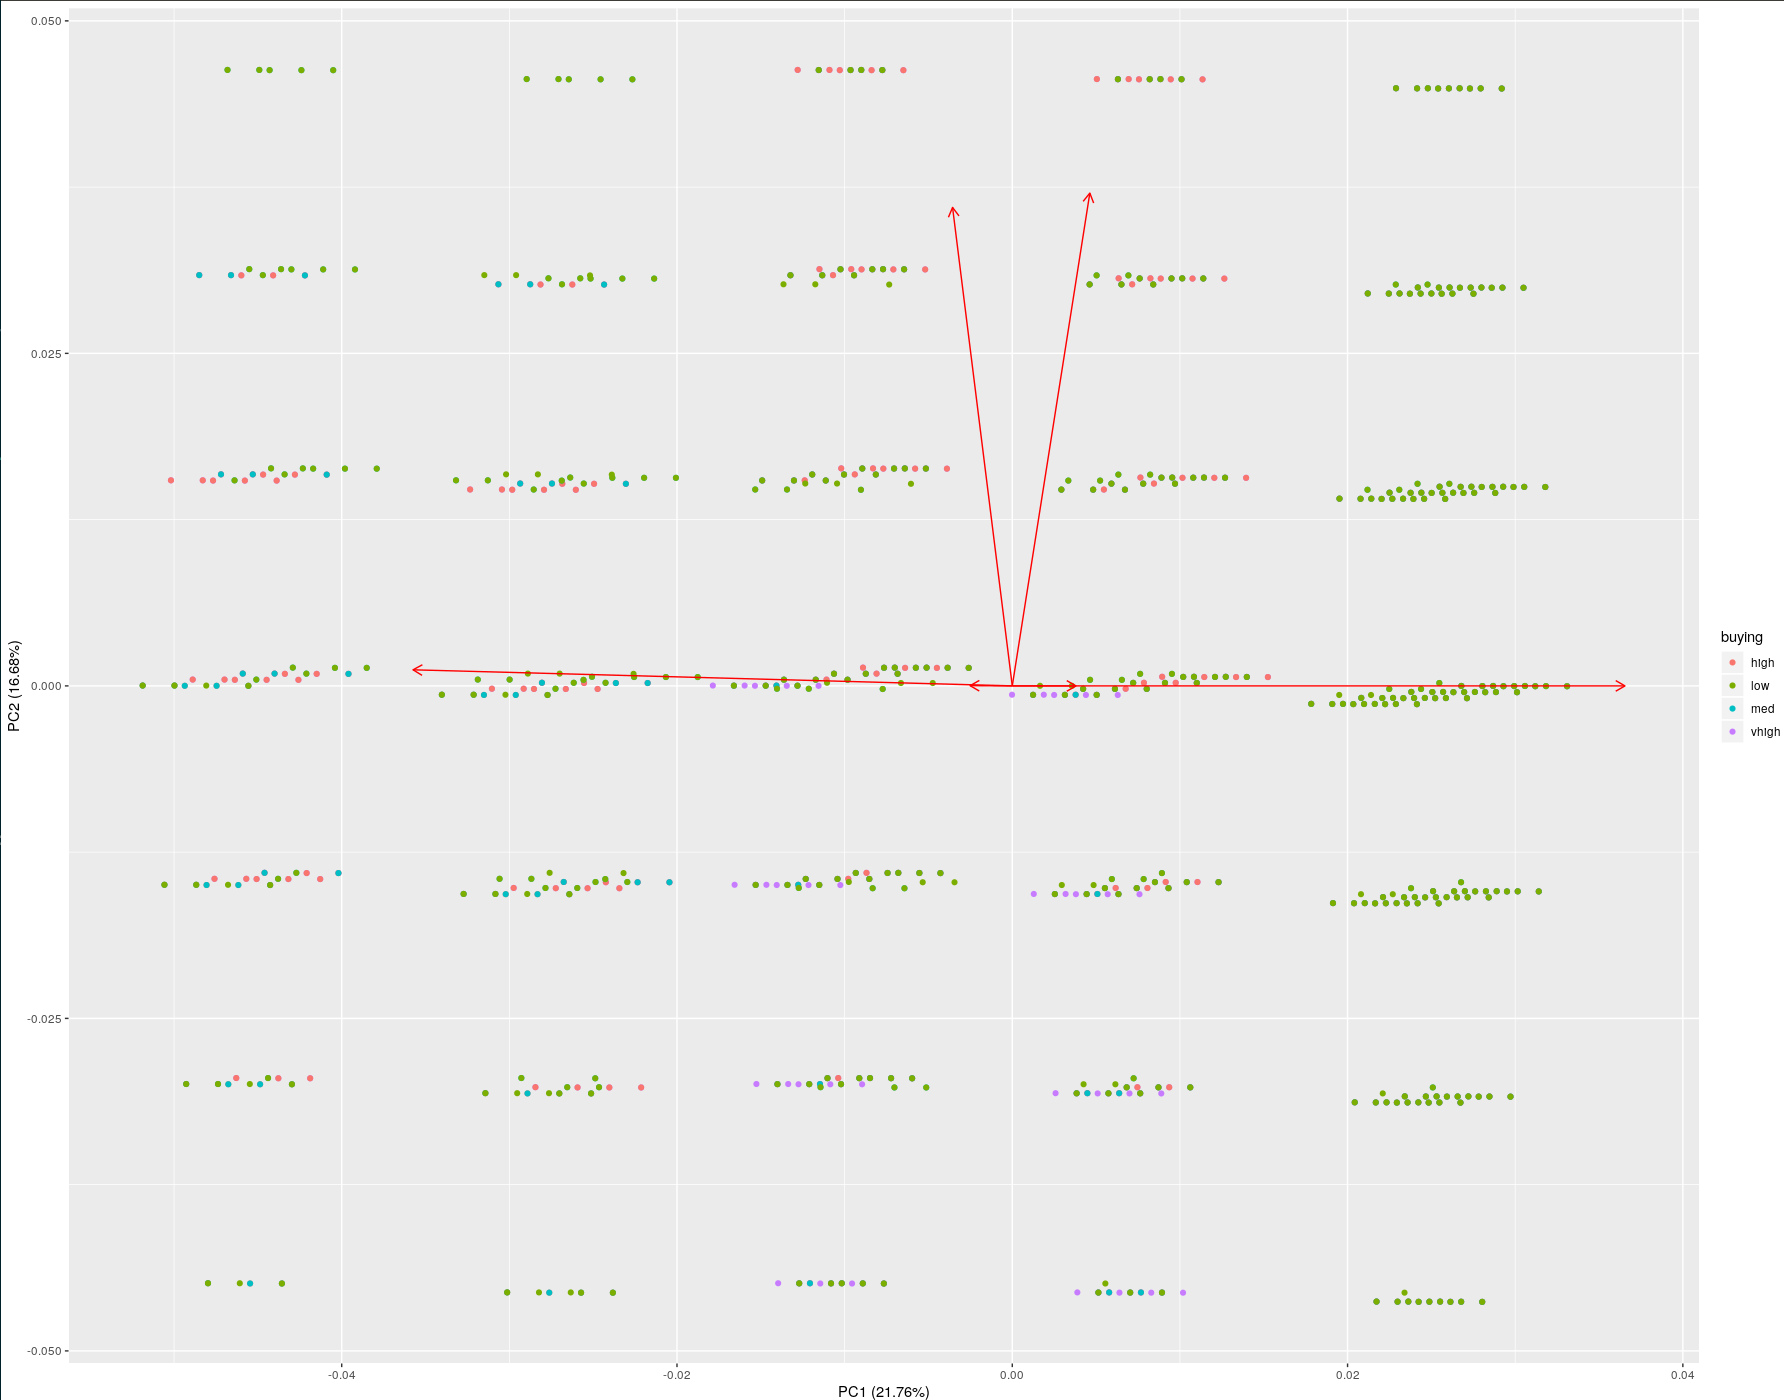
\includegraphics[width=0.6\textwidth]
    {images/PCA-PLOT}
    \caption{PCA plot}
    \label{fig:pca}
  \end{figure}

  As said in the book \cite{modeling-book} having predictors that are not correlated can be advantegous. As you can se on the PCA plot there are not any clusters that sperates the classes.
When trying to train the model using PCA, I get an error rate of 65\%. This is roughly 10\% worse than without PCA. The result might be because the pca has generated componenents that does not capture the relevant data \cite{modeling-book}


\subsection{Between Predictor Correlation}
As i talked about in de Feature Extraction subsection, to high of a correlation is always good for the model accuracy. To remove predictors that are highly correlated we can also use the following algorithm \cite{modeling-book}:
\begin{itemize}
\item Set a treshold
\item Calculate the correlation matrix of the predictors.
\item Find the highest correlation
\item Determine the average correlation between A and all the other variables as well as B.
\item Remove the predictors with the highest average correlation.
\item Repeat this until no predictor correlations are above the treshold you hava set.
\end{itemize}

  \begin{figure}[h]
    \centering 
    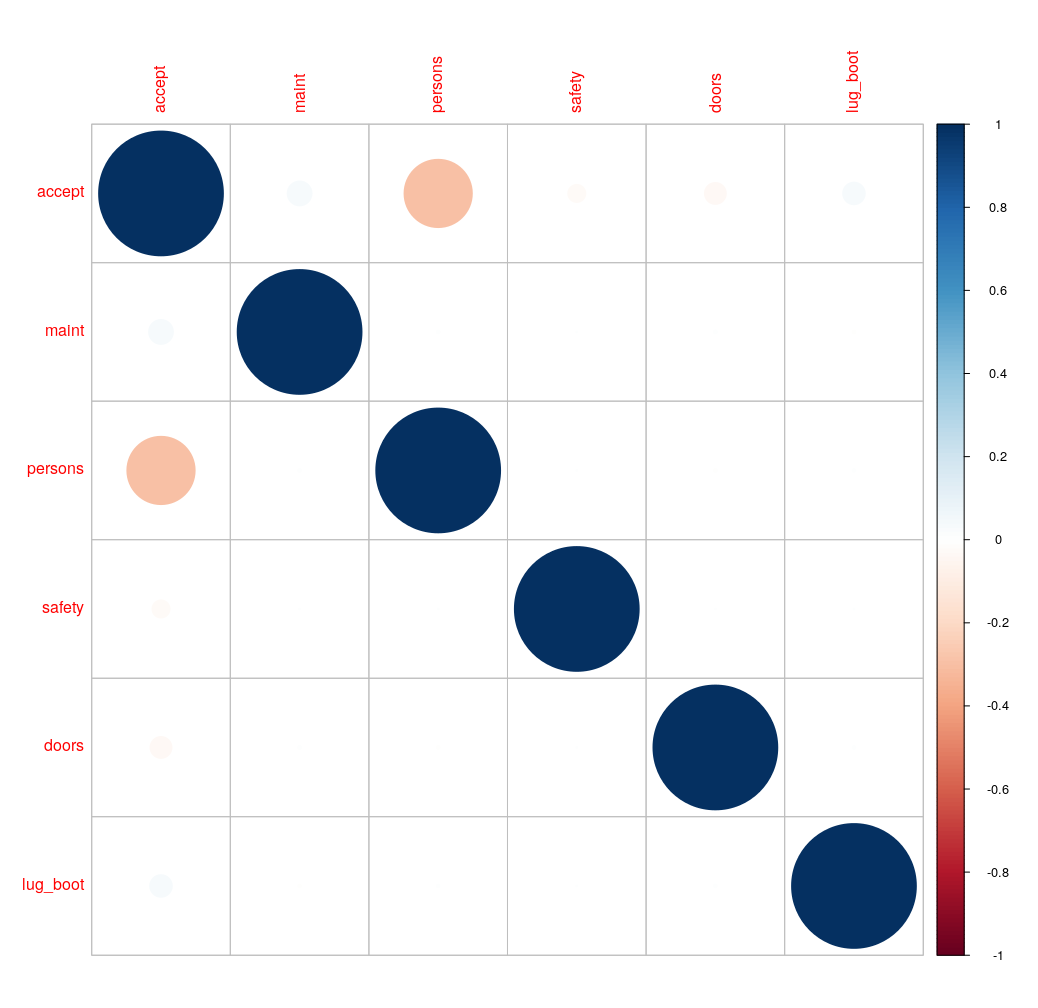
\includegraphics[width=0.6\textwidth]
    {images/correlation}
    \caption{Between predictor correlation}
    \label{fig:correlation}
  \end{figure}

In the car evaluation data set there were no predictors that had a correlation high enough to remove it. This algorithm wil not yield any result for the model.

\section{Classification}
\subsection{C5.0}
I decided to use C5.0 for the classification. It is free and easy use. C5.0 is an algorithm to produce decision trees for classification purposes. For configuring the data and running the algorithm I used R. In R you can use the C5.0 package to generate basic tree-models and rule-based models. In this chapter I will present my findings when using this algorithm on the car evaluation data set. To help me get started with R and the C5.0 algorithm I used this guide \cite{guide}.

\subsection{Findings}
When running the C5.0 algorithm on the car evaluation dateset we found that the accuracy was not very high. We got a 55 percent error rate when using all the predictors. The summary of the first run can bee seen in figure \ref{fig:tree-summary} and the decision tree generated can be seen in figure \ref{fig:decition-tree}.
  \begin{figure}[h]
    \centering 
    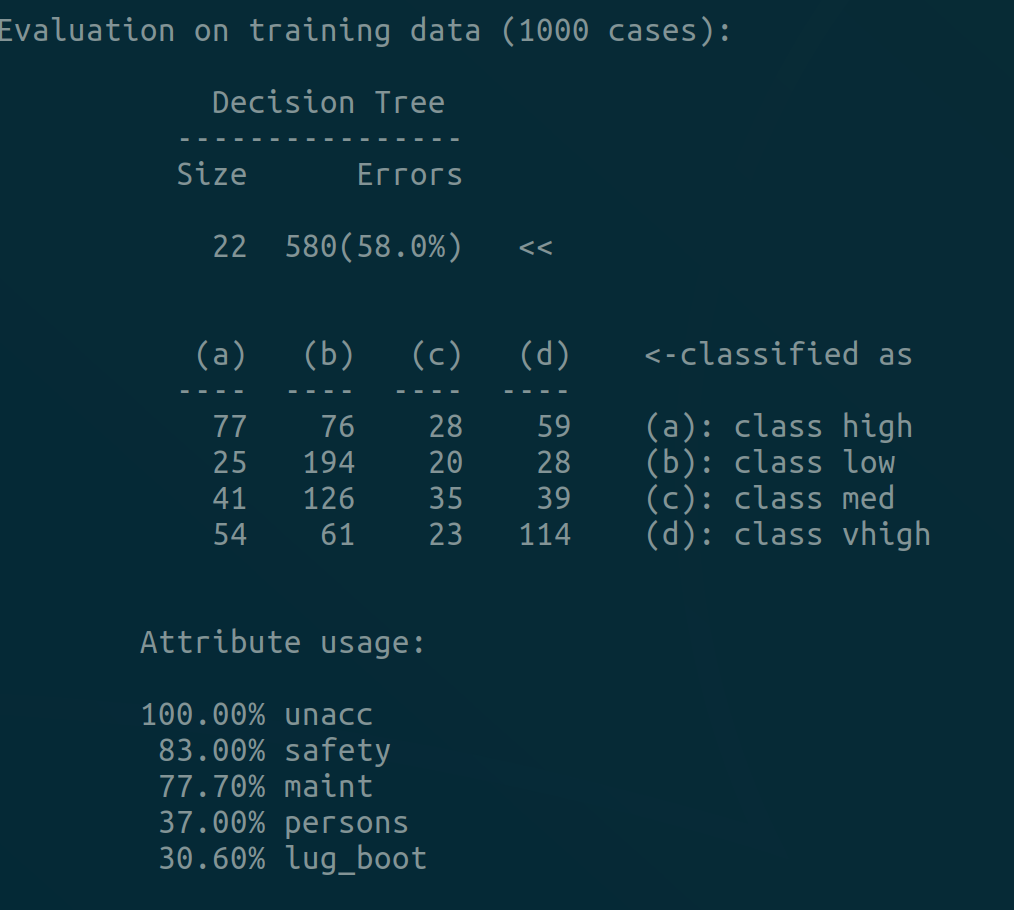
\includegraphics[width=0.6\textwidth]
    {images/summary}
    \caption{tree-summary}
    \label{fig:tree-summary}
  \end{figure}

  \begin{figure}[h]
    \centering 
    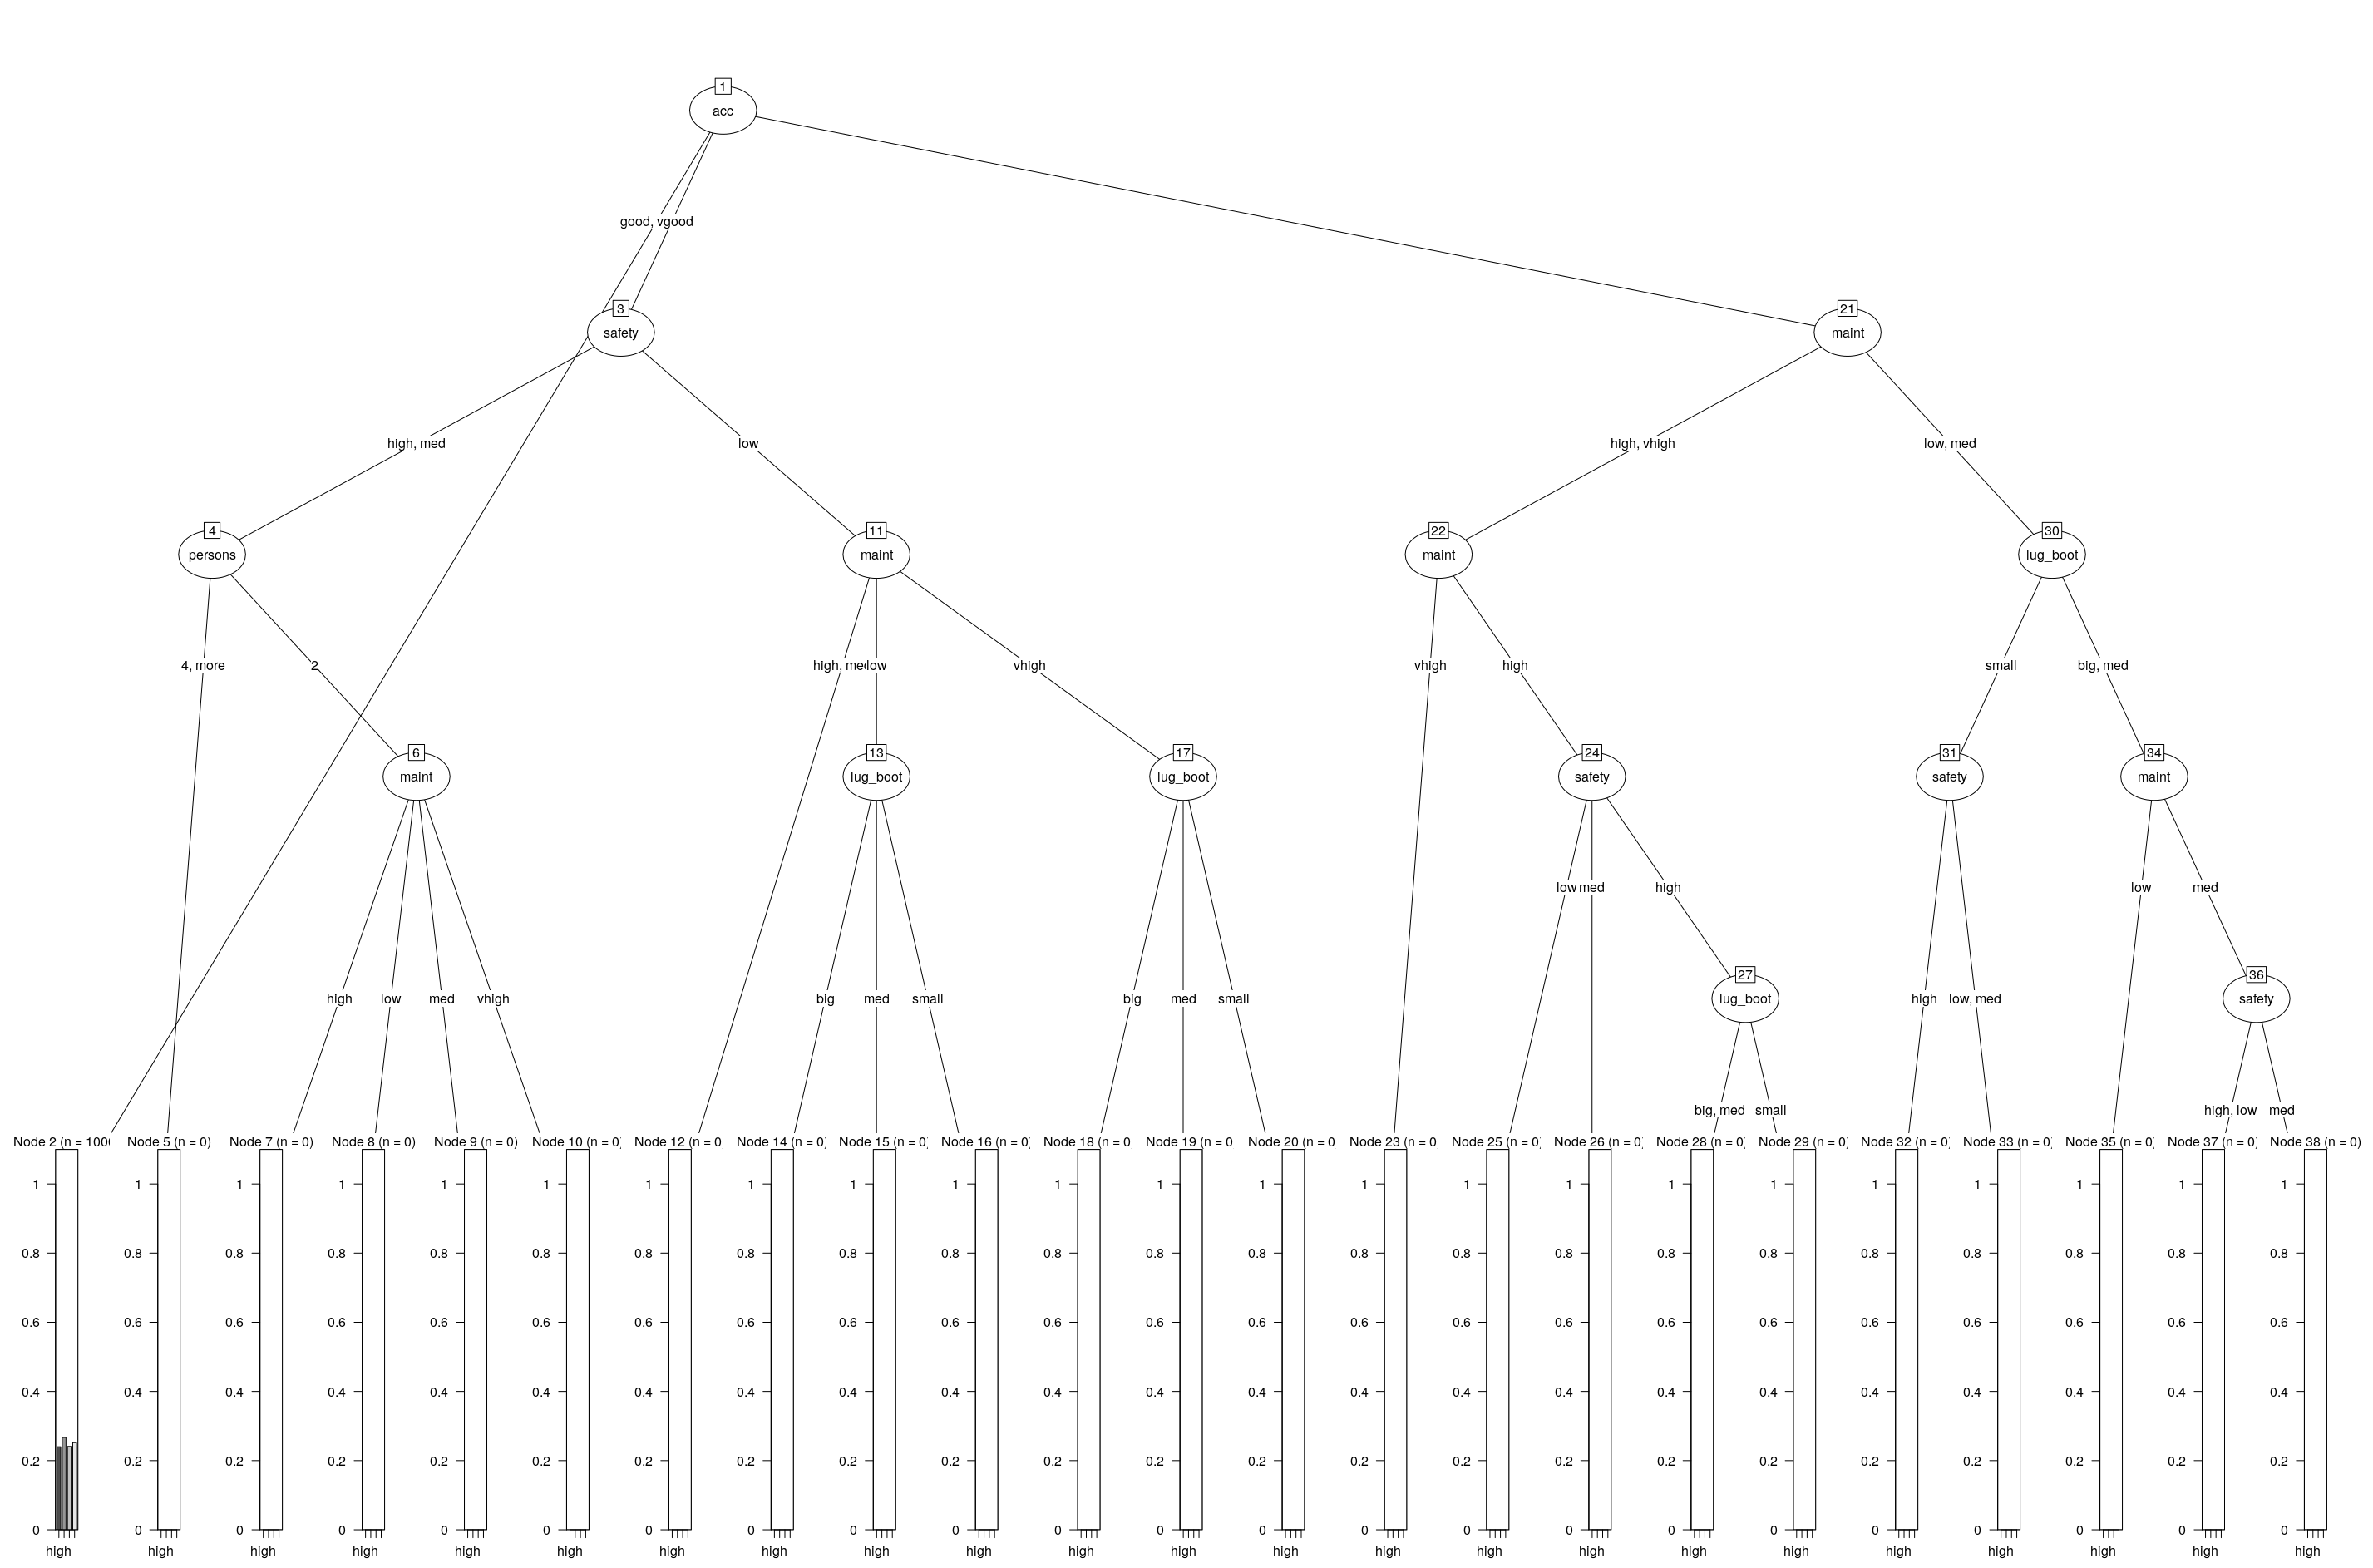
\includegraphics[width=0.6\textwidth]
    {images/tree}
    \caption{Decision-tree}
    \label{fig:decition-tree}
  \end{figure}
  \subsection{Trees and rules}
  When comparing trees in figure \ref{fig:tree-summary} and rules in figure \ref{fig:rules} we see that the error rate is similar. The tree has a slightly better error rate. This is expected because rules are a simplified tree. The rules consists of if-then rules. The rules makes it easier to read, however it might yield a slightly worse result.
  \begin{figure}[h]
    \centering 
    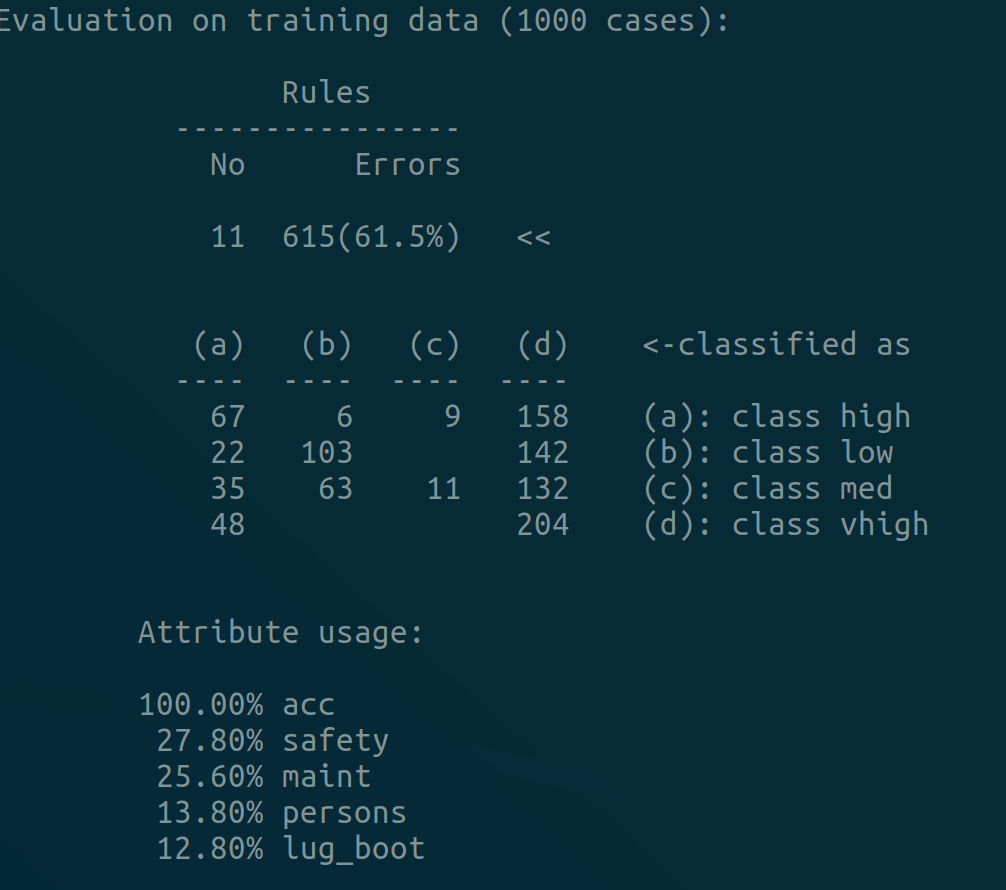
\includegraphics[width=0.6\textwidth]
    {images/summary-rules}
    \caption{Rules}
    \label{fig:rules}
  \end{figure}

  \paragraph{Rules}
  When generating rules from the tree model we get 11 rules or 11 paths through the tree. Some rule are not very sensible like rule number 10 which states that if the car acceptability is unacceptable then the price range is very high. Some rules are more logical like rule 5 that states that if it has medium safety, a small boot size and its in acceptable condition it will be be priced in a low price range.
  Rule 9 also states that if the maintenance costs are medium, it has a big boot and its in acceptable condition it will be priced very high which is very true when it comes to big station wagons or SUV's. This means that some of the rules have logic that someone with domain knowledge can recognize.

  \subsection{Testing the model}
  When I started the building of the model i split the data set. A thousand rows of data was reserved for training the data and 728 rows was reserved for testing. When using the predict function C5.0 on the test data set we get the results displayed in figure \ref{fig:predict}.

  \begin{figure}[h]
    \centering 
    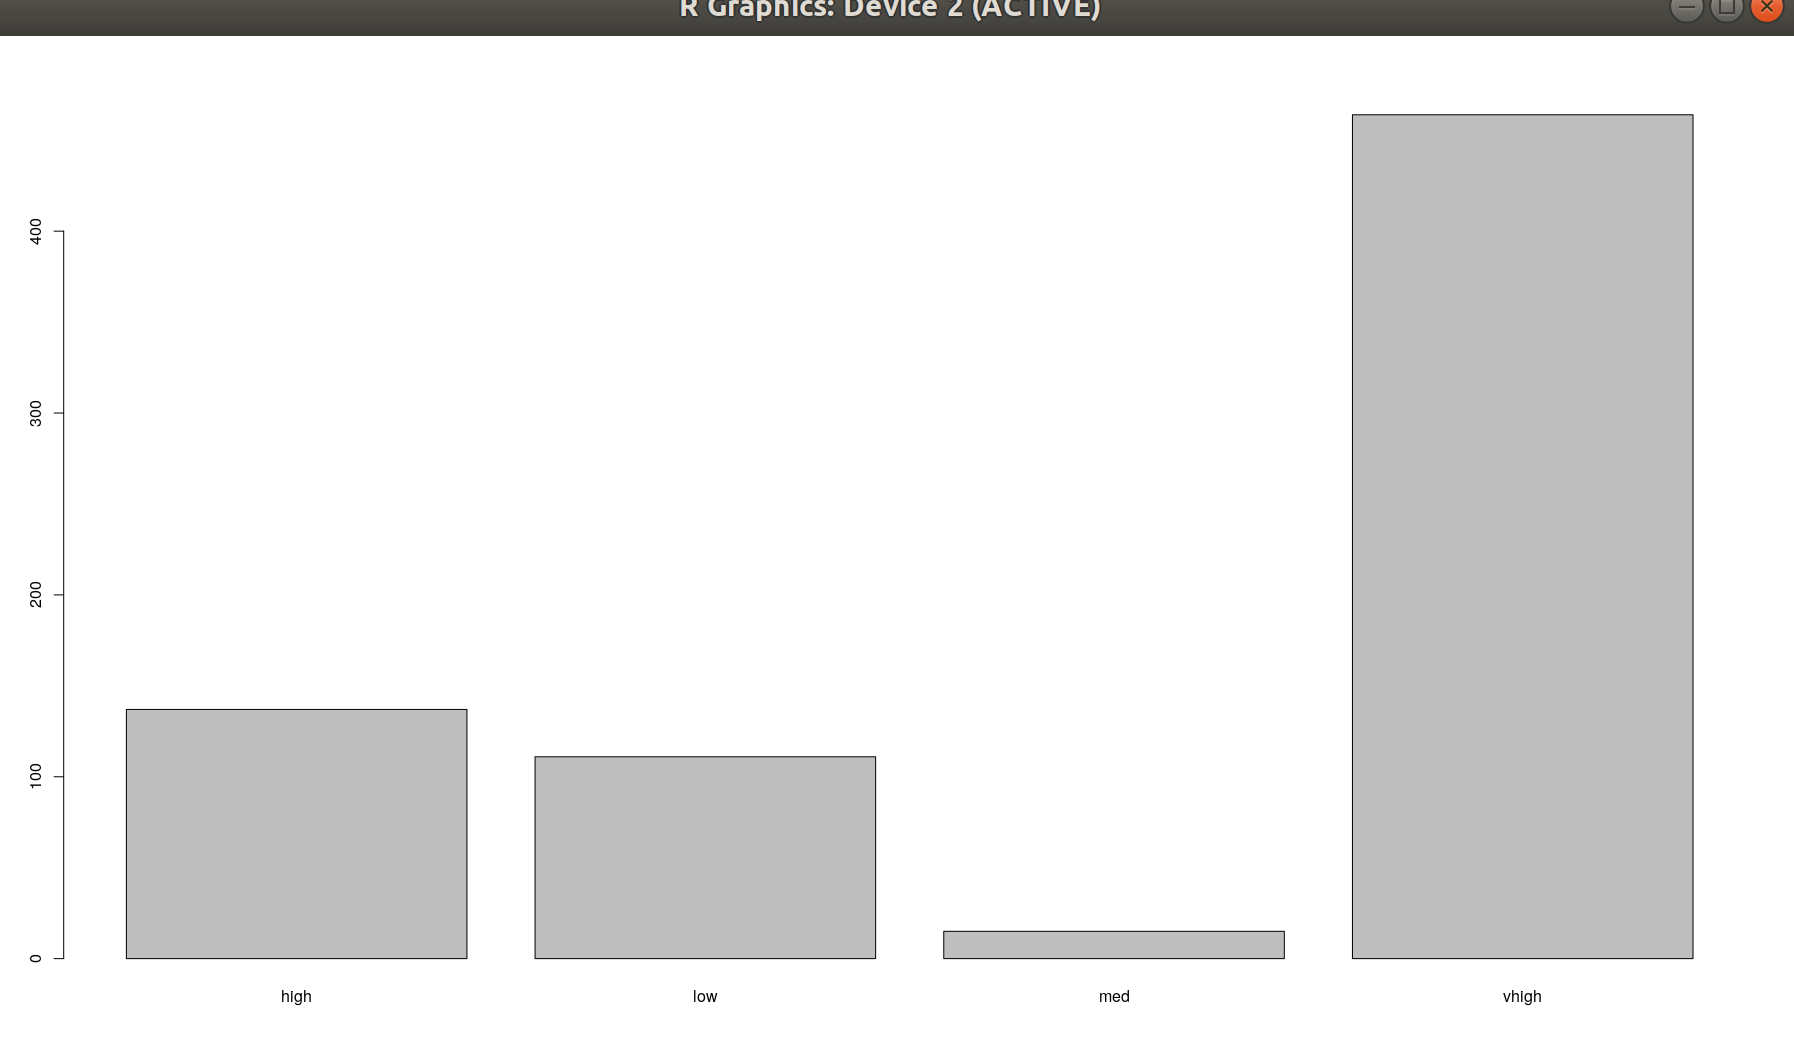
\includegraphics[width=0.8\textwidth]
    {images/predict}
    \caption{Prediction on training set with the rule model}
    \label{fig:predict}
  \end{figure}

  As you can see in figure \ref{fig:predict} the number of cars classified in the v-high price range, way exceed the number of cars that exceed the medium price range. This is expected when you look at the rules of the model. Three ways thorough the tree gives a classification of v-high, but only one classifies it as medium.

  Figure \ref{fig:act} shows the actual distribution.

  \begin{figure}[h]
    \centering 
    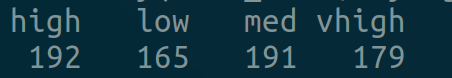
\includegraphics[width=0.8\textwidth]
    {images/actual}
    \caption{Actual distribution of test data}
    \label{fig:act}
  \end{figure}

\subsection{Winnowing, boosting and pruning}
\paragraph{Boosting}
Boosting is an algorithm where multiple model are created. When classifying, all of the models vote for which classification the row will be. I tried to enable boosting for my data set, but it showed up with an error that said that the last classifier was not accurate enough.

\paragraph{Winnowing}
Winnowing is an algorithm that exclude attributes that does not provide any value able information. When i applied the C5.0 algorithm with winnowing enabled it winnowed three attribute, the number of doors, the number of persons that can fit in the car and the boot size. This had a negative effect on the model and the error rate increased with 4.3 percent.

\section{Scikit Learn and dection trees}
\subsection{Trees}
Tree-based models consists of one or more nested if-then statements for the predictors that partition the data.A rule is a set of if-then conditions that have been collapsed into independent conditions.A rule is defined by the tree. A rule is defined as a distinct path through a tree. For the tree, a new sample can only travel down a single path through the tree defined by these rules.Let’s consider an example provided in the book, Applied Predictive Modelling, Chapter 8:If Predictor Ais bigger or equals1.7 then     If predictor B is smaller or equals 202.1 then outcome =1.3. Else outcome =5.6Else outcome = 2.5.

Trees are more sensitive to slight change of parameters. In such cases rules perform rigidly then trees. Rules have there own limitations representing many categories which can be done most effectively by trees.  A  2.5  B  5.6  1.3
Our data set is taken from http://archive.ics.uci.edu/ml/datasets/Car+Evaluation.The dataset is about predicting the model of car (acceptable, unacceptable, very god, good are the class which represents the model). On the basis of features like comfort, buying price, maintenance price, number of doors, number of passengers, luggage boot size, the class of the car is predicted.We model this data set using R and python separately. Here we will discuss aboutthe finding of dataset by using python and decision tree algorithm for classifying the class.In original data set column name was missing. We assign name to each column. During Exploratory Data Analysis, we find that the number of doors were assigned as 5, which is quite unpractical. And, number of People were mentionedas ‘5more’. It was replaced by an integer value of 6. We used Decision Tree Classifier, which is a function of Scikit learn library.

\subsection{Testing}
We split the data set into training and testing set in the proportion of 70\% and 30\% respectively. For the object type attributes of column, dummies variable wasused before fitting the data into Decision tree classifier.

\subsection{Result}
In the figure below you can se the achieved result.


  \begin{figure}[h]
    \centering 
    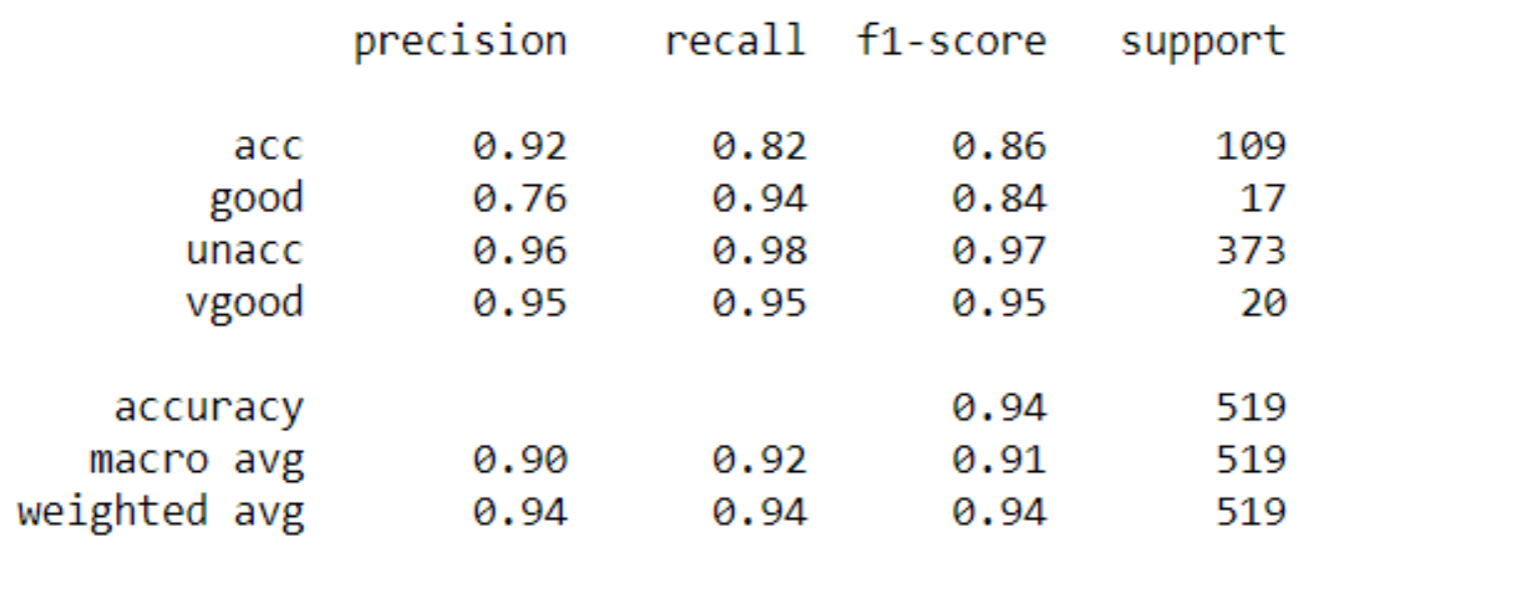
\includegraphics[width=0.8\textwidth]
    {images/confusion}
    \caption{Confusion matrix}
    \label{conf}
  \end{figure}

\section{Conclusion}
In this project i hoped to achieve much greater accuracy than what I did. I have tried the C5.0 algorithm with several configurations and additional algorithms. The best result I was able to achieve was 58 percent error rate. 58 percent in this domain is not satisfactory for the use cases of this model. I have worked systematically Troy try to improve it without no real breakthrough. In order to improve my model I will try other algorithms like XgBoost. I will also try other data set about cars in order to get more predictors to work with. 
\clearpage
\begin{thebibliography}{9}
\bibitem{mml-interference} 
peter J Tan, David L Towe, 2003
\textit{MML Inference of Decision Graphs with Multi-way Joins and Dynamic Attributes
}.

\bibitem{boosting}
  Marc Sebban, Richard Nock, Stéphane Lallich, 2002
  \textit{Stopping Criterion for Boosting-Based Data Reduction Techniques: from Binary to Multiclass Problems}.

\bibitem{learning-set}
  M. Sebban, R. Nock2, J.H. Chauchat and R. Rakotomalala
  \textit{Impact of learning set quality and size on decision tree performance}

\bibitem{dataset}
  Marko Bohanec
  \textit{http://archive.ics.uci.edu/ml/datasets/Car+Evaluation}

\bibitem{dataset-usage}
  Marko Bohanec, Vladislav Rajkovic
  \textit{Knowledge acquisition and explanation for multi-attribute decision making}

\bibitem{guide}
  Rulequest research
  \textit{C5.0: An Informal Tutorial}

\bibitem{modeling-book}
  Max Khun
  \textit{Applied Predictive Modeling}


 
\end{thebibliography}
\end{document}


%%% Local Variables:
%%% mode: latex
%%% TeX-master: t
%%% End:

